\section{UT}

\begin{figure}[htbp]
\begin{center}
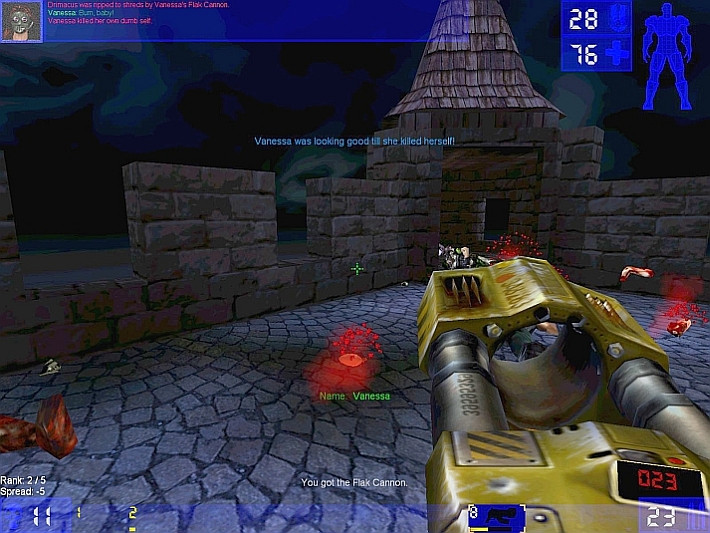
\includegraphics[width=.60\textwidth]{./imagenes/ut.jpg}
\caption{Unreal Tournament}
\label{Unreal Tournament}
\end{center}
\end{figure}
Unreal Tournament \footnote{\url{http://store.steampowered.com/app/13240/}} Unreal Tournament, también conocido como UT y llamado en ocasiones UT99, UT Classic, UT1, o UT:GOTY para diferenciarlo de sus sucesores (Unreal Tournament 2003, Unreal Tournament 2004 y Unreal Tournament 3), es un videojuego de acción en primera persona. 
Lanzado al mercado en 1999, es la continuación del juego Unreal de Epic Games, y su principal enfoque es la acción para multijugador. Compite directamente con el juego Quake III Arena de id Software, que salió al mercado diez días después. Si bien se considera que su competidor tiene mejores gráficos, una buena jugabilidad y un motor gráfico extensamente adoptado, UT tiene una inteligencia artificial superior, una movilidad más variada, y un "disparo alternativo" para las armas, lo que introdujo varios elementos más para la estrategia, más una larga variedad de capacidades multijugador.3

\subsubsection{¿Por qué es uno de mis juegos favoritos?}
\begin{itemize}
\item[Victor Alvarado] La verdad  cuando era pequeño fui a una feria de computacion y vi corriendo castle wolfenstein en una IBM, era lo maximo desde ahi empezo mi gusto por los FPS, siguio los  clasicos como Doom, Doom 2, Heretic, Hexen, Descent , Duke Nukem 3D y unos cuantos mas que son clasicos, pues la competencia empezo.
\end{itemize}